\section{Introduction}

\begin{frame}{Context}
    Our aim is to study, scientifically, the construction of Learning Analytics Dashboards and related software engineering issues.

    \begin{figure}[H]
        \centering
        \label{fig:digital_learning}
        %\caption{The data regarding the student learning process is dispersed across multiple sources} 
        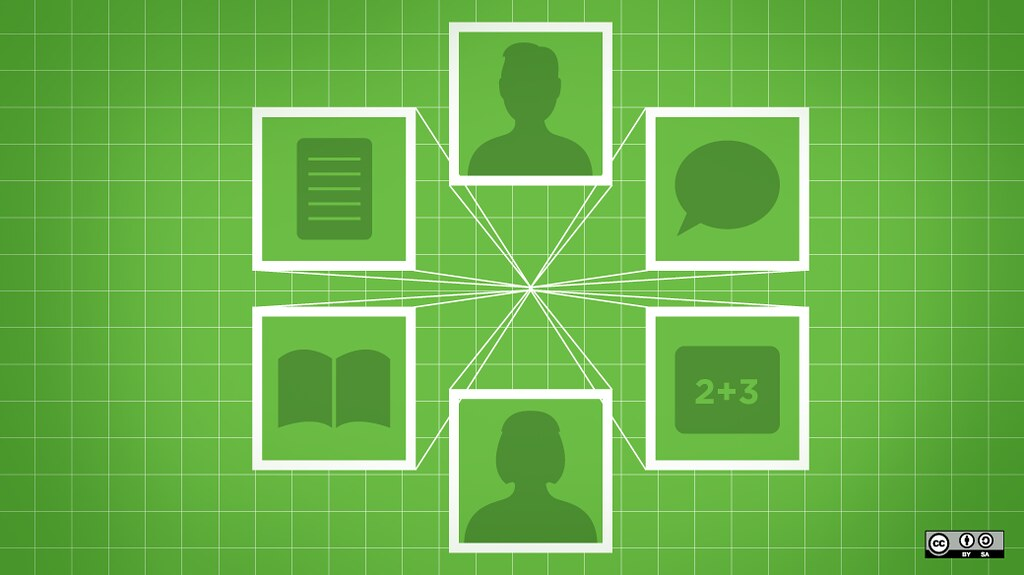
\includegraphics[width=0.5\textwidth]{../../images/digital_learning.jpg}
        \\ \small The data regarding the student learning process is dispersed across multiple sources
        \\ \small \url{https://www.flickr.com/photos/opensourceway/8288335386/}
    \end{figure}

    It is a Learning Analytics research field \cite{lang2017handbook}.
\end{frame}


\begin{frame}{The journey up to this point}
   TIME LINE
\end{frame}

\subsection{Research Questions}
\begin{frame}{Research Questions (temporary yet)}
    \begin{enumerate}[<+-|alert@+>]\color{gray}
        \item What kind of external data can be usefully and safely integrated with 
              the Moodle (behavioral) data?
        \item How this enriched data can be used as features for Statistical and 
              Machine Learning models (to be presented in dashboards) respecting privacy and student autonomy?
    \end{enumerate}
\end{frame}

\begin{frame}{Our proposal}
    The traditional approach used to build dashboards (we are currently confirming through a Systematic Literature Review):

    \begin{table}[]
        \begin{tabular}{|l|l|l|} \hline
                 & Can choose Features? & Can see Predictions?\\ \hline
         Student & No                   & No                  \\ \hline
         Teacher & No                   & Yes                 \\ \hline
         Manager & Yes                  & Yes                 \\ \hline
        \end{tabular}
    \end{table}

    \pause
    Our proposal: Student \underline{in Control} Perspective
    \pause
    \begin{table}[]
        \begin{tabular}{|l|l|l|} \hline
                 & Can choose Features?  & Can see Predictions?                    \\ \hline
         Student & \textcolor{red}{Yes}  & \textcolor{red}{Yes}                    \\ \hline
         Teacher & No                    & \textcolor{blue}{Maybe} (student decides) \\ \hline
         Manager & No                    & \textcolor{blue}{Maybe} (student decides) \\ \hline
        \end{tabular}
    \end{table}

\end{frame}

\begin{frame}{Software Engineering Issues}

    \begin{figure}
        \centering
        \begin{minipage}{.7\textwidth}
            Some issues this approach brings to software engineering:
        \end{minipage}%
        \begin{minipage}{.25\textwidth}
          \centering
          
\includegraphics[width=0.8\textwidth]{../../images/work-workers-men.jpg}
        \end{minipage}
    \end{figure}

    \begin{itemize}[<+-|alert@+>]\color{gray}
        \item The Moodle Analytics API is designed primarily for teachers and managers, so a lot of 
              work is needed on plugins to empower students with similar capabilities
        \item The possibility for each student to choose their own data requires 
              rebuilding the model many times, which can impact performance
    \end{itemize}
\end{frame}

